% ================================================================
% Chapter observation operator (OBS)
% ================================================================
\chapter{Observation and model comparison (OBS)}
\label{OBS}

Authors: D. Lea, M. Martin, K. Mogensen, A. Vidard, A. Weaver, A. Ryan, ...   % do we keep that ?

\minitoc


\newpage
$\ $\newline    % force a new line

The observation and model comparison code (OBS) reads in observation files (profile
temperature and salinity, sea surface temperature, sea level anomaly, sea ice concentration,
and velocity) and calculates  an interpolated model equivalent value at the observation
location and nearest model timestep. The resulting data are saved in a ``feedback'' file (or
files). The code was originally developed for use with the NEMOVAR data assimilation code, but
can be used for validation or verification of model or  any other data assimilation system.

The OBS code is called from \mdl{nemogcm.F90} for model initialisation and to calculate the model
equivalent values for observations on the 0th timestep. The code is then called again after
each timestep from \mdl{step.F90}. To build with the OBS code active \key{diaobs} must be
set.

For all data types a 2D horizontal  interpolator is needed to interpolate the model fields to
the observation location. For {\em in situ} profiles, a 1D vertical interpolator is needed in
addition to provide model fields at the observation depths. Currently this only works in
z-level model configurations, but is being developed to work with a generalised vertical
coordinate system. Temperature data from moored buoys (TAO, TRITON, PIRATA) in the
ENACT/ENSEMBLES data-base are available as daily averaged quantities. For this type of
observation the observation operator will compare such observations to the model temperature
fields averaged over one day. The relevant observation type may be specified in the namelist
using \np{endailyavtypes}. Otherwise the model value from the nearest timestep to the
observation time is used.

The code is controlled by the namelist \textit{nam\_obs}. See the following sections for more
details on setting up the namelist. 

Section~\ref{OBS_example} introduces a test example of the observation operator code including
where to obtain data and how to setup the namelist. Section~\ref{OBS_details} introduces some
more technical details of the different observation types used and also shows a more complete
namelist. Section~\ref{OBS_theory} introduces some of the theoretical aspects of the observation
operator including interpolation methods and running on multiple processors.
Section~\ref{OBS_ooo} describes the offline observation operator code.
Section~\ref{OBS_obsutils} introduces some utilities to help working with the files
produced by the OBS code.

% ================================================================
% Example
% ================================================================
\section{Running the observation operator code example}
\label{OBS_example}

This section describes an example of running the observation operator code using
profile data which can be freely downloaded. It shows how to adapt an
existing run and build of NEMO to run the observation operator.

\begin{enumerate}
\item Compile NEMO with \key{diaobs} set.

\item Download some ENSEMBLES EN3 data from 
\href{http://www.hadobs.org}{http://www.hadobs.org}. Choose observations which are
valid for the period of your test run because the observation operator compares
the model and observations for a matching date and time. 

\item Add the following to the NEMO namelist to run the observation
operator on this data. Set the \np{enactfiles} namelist variable to the
observation  file name:
\end{enumerate}

%------------------------------------------namobs_example-----------------------------------------------------
\namdisplay{namobs_example}
%-------------------------------------------------------------------------------------------------------------

Options are defined through the  \ngn{namobs} namelist variables.
The options \np{ln\_t3d} and \np{ln\_s3d} switch on the temperature and salinity
profile observation operator code. The \np{ln\_ena} switch turns on the reading
of ENACT/ENSEMBLES type profile data. The filename or array of filenames are
specified using the \np{enactfiles} variable. The model grid points for a
particular  observation latitude and longitude are found using the grid
searching part of the code. This can be expensive, particularly for large
numbers of observations, setting \np{ln\_grid\_search\_lookup} allows the use of
a lookup table which is saved into an ``xypos`` file (or files). This will need
to be generated the first time if it does not exist in the run directory.
However, once produced it will significantly speed up future grid searches.
Setting \np{ln\_grid\_global} means that the code distributes the observations
evenly between processors. Alternatively each processor will work with
observations located within the model subdomain (see section~\ref{OBS_parallel}).

A number of utilities are now provided to plot the feedback files, convert and
recombine the files. These are explained in more detail in section~\ref{OBS_obsutils}.

\section{Technical details}
\label{OBS_details}

Here we show a more complete example namelist  \ngn{namobs} and also show the NetCDF headers
of the observation
files that may be used with the observation operator

%------------------------------------------namobs--------------------------------------------------------
\namdisplay{namobs}
%-------------------------------------------------------------------------------------------------------------

This name list uses the "feedback" type observation file input format for
profile, sea level anomaly and sea surface temperature data. All the
observation files must be in NetCDF format. Some example headers (produced using
\mbox{\textit{ncdump~-h}}) for profile
data, sea level anomaly and sea surface temperature are in the following
subsections.

\subsection{Profile feedback type observation file header}

\begin{alltt}
\tiny
\begin{verbatim}
netcdf profiles_01 {
dimensions:
     N_OBS = 603 ;
     N_LEVELS = 150 ;
     N_VARS = 2 ;
     N_QCF = 2 ;
     N_ENTRIES = 1 ;
     N_EXTRA = 1 ;
     STRINGNAM = 8 ;
     STRINGGRID = 1 ;
     STRINGWMO = 8 ;
     STRINGTYP = 4 ;
     STRINGJULD = 14 ;
variables:
     char VARIABLES(N_VARS, STRINGNAM) ;
          VARIABLES:long_name = "List of variables in feedback files" ;
     char ENTRIES(N_ENTRIES, STRINGNAM) ;
          ENTRIES:long_name = "List of additional entries for each variable in feedback files" ;
     char EXTRA(N_EXTRA, STRINGNAM) ;
          EXTRA:long_name = "List of extra variables" ;
     char STATION_IDENTIFIER(N_OBS, STRINGWMO) ;
          STATION_IDENTIFIER:long_name = "Station identifier" ;
     char STATION_TYPE(N_OBS, STRINGTYP) ;
          STATION_TYPE:long_name = "Code instrument type" ;
     double LONGITUDE(N_OBS) ;
          LONGITUDE:long_name = "Longitude" ;
          LONGITUDE:units = "degrees_east" ;
          LONGITUDE:_Fillvalue = 99999.f ;
     double LATITUDE(N_OBS) ;
          LATITUDE:long_name = "Latitude" ;
          LATITUDE:units = "degrees_north" ;
          LATITUDE:_Fillvalue = 99999.f ;
     double DEPTH(N_OBS, N_LEVELS) ;
          DEPTH:long_name = "Depth" ;
          DEPTH:units = "metre" ;
          DEPTH:_Fillvalue = 99999.f ;
     int DEPTH_QC(N_OBS, N_LEVELS) ;
          DEPTH_QC:long_name = "Quality on depth" ;
          DEPTH_QC:Conventions = "q where q =[0,9]" ;
          DEPTH_QC:_Fillvalue = 0 ;
     int DEPTH_QC_FLAGS(N_OBS, N_LEVELS, N_QCF) ;
          DEPTH_QC_FLAGS:long_name = "Quality flags on depth" ;
          DEPTH_QC_FLAGS:Conventions = "NEMOVAR flag conventions" ;
     double JULD(N_OBS) ;
          JULD:long_name = "Julian day" ;
          JULD:units = "days since JULD_REFERENCE" ;
          JULD:Conventions = "relative julian days with decimal part (as parts of day)" ;
          JULD:_Fillvalue = 99999.f ;
     char JULD_REFERENCE(STRINGJULD) ;
          JULD_REFERENCE:long_name = "Date of reference for julian days" ;
          JULD_REFERENCE:Conventions = "YYYYMMDDHHMMSS" ;
     int OBSERVATION_QC(N_OBS) ;
          OBSERVATION_QC:long_name = "Quality on observation" ;
          OBSERVATION_QC:Conventions = "q where q =[0,9]" ;
          OBSERVATION_QC:_Fillvalue = 0 ;
     int OBSERVATION_QC_FLAGS(N_OBS, N_QCF) ;
          OBSERVATION_QC_FLAGS:long_name = "Quality flags on observation" ;
          OBSERVATION_QC_FLAGS:Conventions = "NEMOVAR flag conventions" ;
          OBSERVATION_QC_FLAGS:_Fillvalue = 0 ;
     int POSITION_QC(N_OBS) ;
          POSITION_QC:long_name = "Quality on position (latitude and longitude)" ;
          POSITION_QC:Conventions = "q where q =[0,9]" ;
          POSITION_QC:_Fillvalue = 0 ;
     int POSITION_QC_FLAGS(N_OBS, N_QCF) ;
          POSITION_QC_FLAGS:long_name = "Quality flags on position" ;
          POSITION_QC_FLAGS:Conventions = "NEMOVAR flag conventions" ;
          POSITION_QC_FLAGS:_Fillvalue = 0 ;
     int JULD_QC(N_OBS) ;
          JULD_QC:long_name = "Quality on date and time" ;
          JULD_QC:Conventions = "q where q =[0,9]" ;
          JULD_QC:_Fillvalue = 0 ;
     int JULD_QC_FLAGS(N_OBS, N_QCF) ;
          JULD_QC_FLAGS:long_name = "Quality flags on date and time" ;
          JULD_QC_FLAGS:Conventions = "NEMOVAR flag conventions" ;
          JULD_QC_FLAGS:_Fillvalue = 0 ;
     int ORIGINAL_FILE_INDEX(N_OBS) ;
          ORIGINAL_FILE_INDEX:long_name = "Index in original data file" ;
          ORIGINAL_FILE_INDEX:_Fillvalue = -99999 ;
     float POTM_OBS(N_OBS, N_LEVELS) ;
          POTM_OBS:long_name = "Potential temperature" ;
          POTM_OBS:units = "Degrees Celsius" ;
          POTM_OBS:_Fillvalue = 99999.f ;
     float POTM_Hx(N_OBS, N_LEVELS) ;
          POTM_Hx:long_name = "Model interpolated potential temperature" ;
          POTM_Hx:units = "Degrees Celsius" ;
          POTM_Hx:_Fillvalue = 99999.f ;
     int POTM_QC(N_OBS) ;
          POTM_QC:long_name = "Quality on potential temperature" ;
          POTM_QC:Conventions = "q where q =[0,9]" ;
          POTM_QC:_Fillvalue = 0 ;
     int POTM_QC_FLAGS(N_OBS, N_QCF) ;
          POTM_QC_FLAGS:long_name = "Quality flags on potential temperature" ;
          POTM_QC_FLAGS:Conventions = "NEMOVAR flag conventions" ;
          POTM_QC_FLAGS:_Fillvalue = 0 ;
     int POTM_LEVEL_QC(N_OBS, N_LEVELS) ;
          POTM_LEVEL_QC:long_name = "Quality for each level on potential temperature" ;
          POTM_LEVEL_QC:Conventions = "q where q =[0,9]" ;
          POTM_LEVEL_QC:_Fillvalue = 0 ;
     int POTM_LEVEL_QC_FLAGS(N_OBS, N_LEVELS, N_QCF) ;
          POTM_LEVEL_QC_FLAGS:long_name = "Quality flags for each level on potential temperature" ;
          POTM_LEVEL_QC_FLAGS:Conventions = "NEMOVAR flag conventions" ;
          POTM_LEVEL_QC_FLAGS:_Fillvalue = 0 ;
     int POTM_IOBSI(N_OBS) ;
          POTM_IOBSI:long_name = "ORCA grid search I coordinate" ;
     int POTM_IOBSJ(N_OBS) ;
          POTM_IOBSJ:long_name = "ORCA grid search J coordinate" ;
     int POTM_IOBSK(N_OBS, N_LEVELS) ;
          POTM_IOBSK:long_name = "ORCA grid search K coordinate" ;
     char POTM_GRID(STRINGGRID) ;
          POTM_GRID:long_name = "ORCA grid search grid (T,U,V)" ;
     float PSAL_OBS(N_OBS, N_LEVELS) ;
          PSAL_OBS:long_name = "Practical salinity" ;
          PSAL_OBS:units = "PSU" ;
          PSAL_OBS:_Fillvalue = 99999.f ;
     float PSAL_Hx(N_OBS, N_LEVELS) ;
          PSAL_Hx:long_name = "Model interpolated practical salinity" ;
          PSAL_Hx:units = "PSU" ;
          PSAL_Hx:_Fillvalue = 99999.f ;
     int PSAL_QC(N_OBS) ;
          PSAL_QC:long_name = "Quality on practical salinity" ;
          PSAL_QC:Conventions = "q where q =[0,9]" ;
          PSAL_QC:_Fillvalue = 0 ;
     int PSAL_QC_FLAGS(N_OBS, N_QCF) ;
          PSAL_QC_FLAGS:long_name = "Quality flags on practical salinity" ;
          PSAL_QC_FLAGS:Conventions = "NEMOVAR flag conventions" ;
          PSAL_QC_FLAGS:_Fillvalue = 0 ;
     int PSAL_LEVEL_QC(N_OBS, N_LEVELS) ;
          PSAL_LEVEL_QC:long_name = "Quality for each level on practical salinity" ;
          PSAL_LEVEL_QC:Conventions = "q where q =[0,9]" ;
          PSAL_LEVEL_QC:_Fillvalue = 0 ;
     int PSAL_LEVEL_QC_FLAGS(N_OBS, N_LEVELS, N_QCF) ;
          PSAL_LEVEL_QC_FLAGS:long_name = "Quality flags for each level on practical salinity" ;
          PSAL_LEVEL_QC_FLAGS:Conventions = "NEMOVAR flag conventions" ;
          PSAL_LEVEL_QC_FLAGS:_Fillvalue = 0 ;
     int PSAL_IOBSI(N_OBS) ;
          PSAL_IOBSI:long_name = "ORCA grid search I coordinate" ;
     int PSAL_IOBSJ(N_OBS) ;
          PSAL_IOBSJ:long_name = "ORCA grid search J coordinate" ;
     int PSAL_IOBSK(N_OBS, N_LEVELS) ;
          PSAL_IOBSK:long_name = "ORCA grid search K coordinate" ;
     char PSAL_GRID(STRINGGRID) ;
          PSAL_GRID:long_name = "ORCA grid search grid (T,U,V)" ;
     float TEMP(N_OBS, N_LEVELS) ;
          TEMP:long_name = "Insitu temperature" ;
          TEMP:units = "Degrees Celsius" ;
          TEMP:_Fillvalue = 99999.f ;

// global attributes:
          :title = "NEMO observation operator output" ;
          :Convention = "NEMO unified observation operator output" ;
}
\end{verbatim}
\end{alltt}

\subsection{Sea level anomaly feedback type observation file header}

\begin{alltt}
\tiny
\begin{verbatim}
netcdf sla_01 {
dimensions:
     N_OBS = 41301 ;
     N_LEVELS = 1 ;
     N_VARS = 1 ;
     N_QCF = 2 ;
     N_ENTRIES = 1 ;
     N_EXTRA = 1 ;
     STRINGNAM = 8 ;
     STRINGGRID = 1 ;
     STRINGWMO = 8 ;
     STRINGTYP = 4 ;
     STRINGJULD = 14 ;
variables:
     char VARIABLES(N_VARS, STRINGNAM) ;
          VARIABLES:long_name = "List of variables in feedback files" ;
     char ENTRIES(N_ENTRIES, STRINGNAM) ;
          ENTRIES:long_name = "List of additional entries for each variable in feedback files" ;
     char EXTRA(N_EXTRA, STRINGNAM) ;
          EXTRA:long_name = "List of extra variables" ;
     char STATION_IDENTIFIER(N_OBS, STRINGWMO) ;
          STATION_IDENTIFIER:long_name = "Station identifier" ;
     char STATION_TYPE(N_OBS, STRINGTYP) ;
          STATION_TYPE:long_name = "Code instrument type" ;
     double LONGITUDE(N_OBS) ;
          LONGITUDE:long_name = "Longitude" ;
          LONGITUDE:units = "degrees_east" ;
          LONGITUDE:_Fillvalue = 99999.f ;
     double LATITUDE(N_OBS) ;
          LATITUDE:long_name = "Latitude" ;
          LATITUDE:units = "degrees_north" ;
          LATITUDE:_Fillvalue = 99999.f ;
     double DEPTH(N_OBS, N_LEVELS) ;
          DEPTH:long_name = "Depth" ;
          DEPTH:units = "metre" ;
          DEPTH:_Fillvalue = 99999.f ;
     int DEPTH_QC(N_OBS, N_LEVELS) ;
          DEPTH_QC:long_name = "Quality on depth" ;
          DEPTH_QC:Conventions = "q where q =[0,9]" ;
          DEPTH_QC:_Fillvalue = 0 ;
     int DEPTH_QC_FLAGS(N_OBS, N_LEVELS, N_QCF) ;
          DEPTH_QC_FLAGS:long_name = "Quality flags on depth" ;
          DEPTH_QC_FLAGS:Conventions = "NEMOVAR flag conventions" ;
     double JULD(N_OBS) ;
          JULD:long_name = "Julian day" ;
          JULD:units = "days since JULD_REFERENCE" ;
          JULD:Conventions = "relative julian days with decimal part (as parts of day)" ;
          JULD:_Fillvalue = 99999.f ;
     char JULD_REFERENCE(STRINGJULD) ;
          JULD_REFERENCE:long_name = "Date of reference for julian days" ;
          JULD_REFERENCE:Conventions = "YYYYMMDDHHMMSS" ;
     int OBSERVATION_QC(N_OBS) ;
          OBSERVATION_QC:long_name = "Quality on observation" ;
          OBSERVATION_QC:Conventions = "q where q =[0,9]" ;
          OBSERVATION_QC:_Fillvalue = 0 ;
     int OBSERVATION_QC_FLAGS(N_OBS, N_QCF) ;
          OBSERVATION_QC_FLAGS:long_name = "Quality flags on observation" ;
          OBSERVATION_QC_FLAGS:Conventions = "NEMOVAR flag conventions" ;
          OBSERVATION_QC_FLAGS:_Fillvalue = 0 ;
     int POSITION_QC(N_OBS) ;
          POSITION_QC:long_name = "Quality on position (latitude and longitude)" ;
          POSITION_QC:Conventions = "q where q =[0,9]" ;
          POSITION_QC:_Fillvalue = 0 ;
     int POSITION_QC_FLAGS(N_OBS, N_QCF) ;
          POSITION_QC_FLAGS:long_name = "Quality flags on position" ;
          POSITION_QC_FLAGS:Conventions = "NEMOVAR flag conventions" ;
          POSITION_QC_FLAGS:_Fillvalue = 0 ;
     int JULD_QC(N_OBS) ;
          JULD_QC:long_name = "Quality on date and time" ;
          JULD_QC:Conventions = "q where q =[0,9]" ;
          JULD_QC:_Fillvalue = 0 ;
     int JULD_QC_FLAGS(N_OBS, N_QCF) ;
          JULD_QC_FLAGS:long_name = "Quality flags on date and time" ;
          JULD_QC_FLAGS:Conventions = "NEMOVAR flag conventions" ;
          JULD_QC_FLAGS:_Fillvalue = 0 ;
     int ORIGINAL_FILE_INDEX(N_OBS) ;
          ORIGINAL_FILE_INDEX:long_name = "Index in original data file" ;
          ORIGINAL_FILE_INDEX:_Fillvalue = -99999 ;
     float SLA_OBS(N_OBS, N_LEVELS) ;
          SLA_OBS:long_name = "Sea level anomaly" ;
          SLA_OBS:units = "metre" ;
          SLA_OBS:_Fillvalue = 99999.f ;
     float SLA_Hx(N_OBS, N_LEVELS) ;
          SLA_Hx:long_name = "Model interpolated sea level anomaly" ;
          SLA_Hx:units = "metre" ;
          SLA_Hx:_Fillvalue = 99999.f ;
     int SLA_QC(N_OBS) ;
          SLA_QC:long_name = "Quality on sea level anomaly" ;
          SLA_QC:Conventions = "q where q =[0,9]" ;
          SLA_QC:_Fillvalue = 0 ;
     int SLA_QC_FLAGS(N_OBS, N_QCF) ;
          SLA_QC_FLAGS:long_name = "Quality flags on sea level anomaly" ;
          SLA_QC_FLAGS:Conventions = "NEMOVAR flag conventions" ;
          SLA_QC_FLAGS:_Fillvalue = 0 ;
     int SLA_LEVEL_QC(N_OBS, N_LEVELS) ;
          SLA_LEVEL_QC:long_name = "Quality for each level on sea level anomaly" ;
          SLA_LEVEL_QC:Conventions = "q where q =[0,9]" ;
          SLA_LEVEL_QC:_Fillvalue = 0 ;
     int SLA_LEVEL_QC_FLAGS(N_OBS, N_LEVELS, N_QCF) ;
          SLA_LEVEL_QC_FLAGS:long_name = "Quality flags for each level on sea level anomaly" ;
          SLA_LEVEL_QC_FLAGS:Conventions = "NEMOVAR flag conventions" ;
          SLA_LEVEL_QC_FLAGS:_Fillvalue = 0 ;
     int SLA_IOBSI(N_OBS) ;
          SLA_IOBSI:long_name = "ORCA grid search I coordinate" ;
     int SLA_IOBSJ(N_OBS) ;
          SLA_IOBSJ:long_name = "ORCA grid search J coordinate" ;
     int SLA_IOBSK(N_OBS, N_LEVELS) ;
          SLA_IOBSK:long_name = "ORCA grid search K coordinate" ;
     char SLA_GRID(STRINGGRID) ;
          SLA_GRID:long_name = "ORCA grid search grid (T,U,V)" ;
     float MDT(N_OBS, N_LEVELS) ;
          MDT:long_name = "Mean Dynamic Topography" ;
          MDT:units = "metre" ;
          MDT:_Fillvalue = 99999.f ;

// global attributes:
          :title = "NEMO observation operator output" ;
          :Convention = "NEMO unified observation operator output" ;
}
\end{verbatim}
\end{alltt}

The mean dynamic
topography (MDT) must be provided in a separate file defined on the model grid
 called {\it slaReferenceLevel.nc}. The MDT is required in
order to produce the model equivalent sea level anomaly from the model sea
surface height. Below is an example header for this file (on the ORCA025 grid).

\begin{alltt}
\tiny
\begin{verbatim}
dimensions:
        x = 1442 ;
        y = 1021 ;
variables:
        float nav_lon(y, x) ;
                nav_lon:units = "degrees_east" ;
        float nav_lat(y, x) ;
                nav_lat:units = "degrees_north" ;
        float sossheig(y, x) ;
                sossheig:_FillValue = -1.e+30f ;
                sossheig:coordinates = "nav_lon nav_lat" ;
                sossheig:long_name = "Mean Dynamic Topography" ;
                sossheig:units = "metres" ;
                sossheig:grid = "orca025T" ;
\end{verbatim}
\end{alltt}

\subsection{Sea surface temperature feedback type observation file header}

\begin{alltt}
\tiny
\begin{verbatim}
netcdf sst_01 {
dimensions:
     N_OBS = 33099 ;
     N_LEVELS = 1 ;
     N_VARS = 1 ;
     N_QCF = 2 ;
     N_ENTRIES = 1 ;
     STRINGNAM = 8 ;
     STRINGGRID = 1 ;
     STRINGWMO = 8 ;
     STRINGTYP = 4 ;
     STRINGJULD = 14 ;
variables:
     char VARIABLES(N_VARS, STRINGNAM) ;
          VARIABLES:long_name = "List of variables in feedback files" ;
     char ENTRIES(N_ENTRIES, STRINGNAM) ;
          ENTRIES:long_name = "List of additional entries for each variable in feedback files" ;
     char STATION_IDENTIFIER(N_OBS, STRINGWMO) ;
          STATION_IDENTIFIER:long_name = "Station identifier" ;
     char STATION_TYPE(N_OBS, STRINGTYP) ;
          STATION_TYPE:long_name = "Code instrument type" ;
     double LONGITUDE(N_OBS) ;
          LONGITUDE:long_name = "Longitude" ;
          LONGITUDE:units = "degrees_east" ;
          LONGITUDE:_Fillvalue = 99999.f ;
     double LATITUDE(N_OBS) ;
          LATITUDE:long_name = "Latitude" ;
          LATITUDE:units = "degrees_north" ;
          LATITUDE:_Fillvalue = 99999.f ;
     double DEPTH(N_OBS, N_LEVELS) ;
          DEPTH:long_name = "Depth" ;
          DEPTH:units = "metre" ;
          DEPTH:_Fillvalue = 99999.f ;
     int DEPTH_QC(N_OBS, N_LEVELS) ;
          DEPTH_QC:long_name = "Quality on depth" ;
          DEPTH_QC:Conventions = "q where q =[0,9]" ;
          DEPTH_QC:_Fillvalue = 0 ;
     int DEPTH_QC_FLAGS(N_OBS, N_LEVELS, N_QCF) ;
          DEPTH_QC_FLAGS:long_name = "Quality flags on depth" ;
          DEPTH_QC_FLAGS:Conventions = "NEMOVAR flag conventions" ;
     double JULD(N_OBS) ;
          JULD:long_name = "Julian day" ;
          JULD:units = "days since JULD_REFERENCE" ;
          JULD:Conventions = "relative julian days with decimal part (as parts of day)" ;
          JULD:_Fillvalue = 99999.f ;
     char JULD_REFERENCE(STRINGJULD) ;
          JULD_REFERENCE:long_name = "Date of reference for julian days" ;
          JULD_REFERENCE:Conventions = "YYYYMMDDHHMMSS" ;
     int OBSERVATION_QC(N_OBS) ;
          OBSERVATION_QC:long_name = "Quality on observation" ;
          OBSERVATION_QC:Conventions = "q where q =[0,9]" ;
          OBSERVATION_QC:_Fillvalue = 0 ;
     int OBSERVATION_QC_FLAGS(N_OBS, N_QCF) ;
          OBSERVATION_QC_FLAGS:long_name = "Quality flags on observation" ;
          OBSERVATION_QC_FLAGS:Conventions = "NEMOVAR flag conventions" ;
          OBSERVATION_QC_FLAGS:_Fillvalue = 0 ;
     int POSITION_QC(N_OBS) ;
          POSITION_QC:long_name = "Quality on position (latitude and longitude)" ;
          POSITION_QC:Conventions = "q where q =[0,9]" ;
          POSITION_QC:_Fillvalue = 0 ;
     int POSITION_QC_FLAGS(N_OBS, N_QCF) ;
          POSITION_QC_FLAGS:long_name = "Quality flags on position" ;
          POSITION_QC_FLAGS:Conventions = "NEMOVAR flag conventions" ;
          POSITION_QC_FLAGS:_Fillvalue = 0 ;
     int JULD_QC(N_OBS) ;
          JULD_QC:long_name = "Quality on date and time" ;
          JULD_QC:Conventions = "q where q =[0,9]" ;
          JULD_QC:_Fillvalue = 0 ;
     int JULD_QC_FLAGS(N_OBS, N_QCF) ;
          JULD_QC_FLAGS:long_name = "Quality flags on date and time" ;
          JULD_QC_FLAGS:Conventions = "NEMOVAR flag conventions" ;
          JULD_QC_FLAGS:_Fillvalue = 0 ;
     int ORIGINAL_FILE_INDEX(N_OBS) ;
          ORIGINAL_FILE_INDEX:long_name = "Index in original data file" ;
          ORIGINAL_FILE_INDEX:_Fillvalue = -99999 ;
     float SST_OBS(N_OBS, N_LEVELS) ;
          SST_OBS:long_name = "Sea surface temperature" ;
          SST_OBS:units = "Degree centigrade" ;
          SST_OBS:_Fillvalue = 99999.f ;
     float SST_Hx(N_OBS, N_LEVELS) ;
          SST_Hx:long_name = "Model interpolated sea surface temperature" ;
          SST_Hx:units = "Degree centigrade" ;
          SST_Hx:_Fillvalue = 99999.f ;
     int SST_QC(N_OBS) ;
          SST_QC:long_name = "Quality on sea surface temperature" ;
          SST_QC:Conventions = "q where q =[0,9]" ;
          SST_QC:_Fillvalue = 0 ;
     int SST_QC_FLAGS(N_OBS, N_QCF) ;
          SST_QC_FLAGS:long_name = "Quality flags on sea surface temperature" ;
          SST_QC_FLAGS:Conventions = "NEMOVAR flag conventions" ;
          SST_QC_FLAGS:_Fillvalue = 0 ;
     int SST_LEVEL_QC(N_OBS, N_LEVELS) ;
          SST_LEVEL_QC:long_name = "Quality for each level on sea surface temperature" ;
          SST_LEVEL_QC:Conventions = "q where q =[0,9]" ;
          SST_LEVEL_QC:_Fillvalue = 0 ;
     int SST_LEVEL_QC_FLAGS(N_OBS, N_LEVELS, N_QCF) ;
          SST_LEVEL_QC_FLAGS:long_name = "Quality flags for each level on sea surface temperature" ;
          SST_LEVEL_QC_FLAGS:Conventions = "NEMOVAR flag conventions" ;
          SST_LEVEL_QC_FLAGS:_Fillvalue = 0 ;
     int SST_IOBSI(N_OBS) ;
          SST_IOBSI:long_name = "ORCA grid search I coordinate" ;
     int SST_IOBSJ(N_OBS) ;
          SST_IOBSJ:long_name = "ORCA grid search J coordinate" ;
     int SST_IOBSK(N_OBS, N_LEVELS) ;
          SST_IOBSK:long_name = "ORCA grid search K coordinate" ;
     char SST_GRID(STRINGGRID) ;
          SST_GRID:long_name = "ORCA grid search grid (T,U,V)" ;

// global attributes:
          :title = "NEMO observation operator output" ;
          :Convention = "NEMO unified observation operator output" ;
}
\end{verbatim}
\end{alltt}

\section{Theoretical details}
\label{OBS_theory}

\subsection{Horizontal interpolation methods}

Consider an observation point ${\rm P}$ with 
with longitude and latitude $({\lambda_{}}_{\rm P}, \phi_{\rm P})$ and the 
four nearest neighbouring model grid points ${\rm A}$, ${\rm B}$, ${\rm C}$ 
and ${\rm D}$ with longitude and latitude ($\lambda_{\rm A}$, $\phi_{\rm A}$),
($\lambda_{\rm B}$, $\phi_{\rm B}$) etc.
All horizontal interpolation methods implemented in NEMO
estimate the value of a model variable $x$ at point $P$ as
a weighted linear combination of the values of the model 
variables at the grid points ${\rm A}$, ${\rm B}$ etc.:
\begin{eqnarray}
{x_{}}_{\rm P} & \hspace{-2mm} = \hspace{-2mm} & 
\frac{1}{w} \left( {w_{}}_{\rm A} {x_{}}_{\rm A} + 
                   {w_{}}_{\rm B} {x_{}}_{\rm B} + 
                   {w_{}}_{\rm C} {x_{}}_{\rm C} + 
                   {w_{}}_{\rm D} {x_{}}_{\rm D} \right)
\end{eqnarray}
where ${w_{}}_{\rm A}$, ${w_{}}_{\rm B}$ etc. are the respective weights for the 
model field at points ${\rm A}$, ${\rm B}$ etc., and 
$w = {w_{}}_{\rm A} + {w_{}}_{\rm B} + {w_{}}_{\rm C} + {w_{}}_{\rm D}$.

Four different possibilities are available for computing the weights.

\begin{enumerate}

\item[1.] {\bf Great-Circle distance-weighted interpolation.} The weights
  are computed as a function of the great-circle distance $s(P, \cdot)$ 
  between $P$ and the model grid points $A$, $B$ etc. For example, 
  the weight given to the field ${x_{}}_{\rm A}$ is specified as the 
  product of the distances from ${\rm P}$ to the other points:
  \begin{eqnarray}
  {w_{}}_{\rm A} = s({\rm P}, {\rm B}) \, s({\rm P}, {\rm C}) \, s({\rm P}, {\rm D})
  \nonumber
  \end{eqnarray}
  where 
  \begin{eqnarray}
   s\left ({\rm P}, {\rm M} \right ) 
     & \hspace{-2mm} = \hspace{-2mm} & 
      \cos^{-1} \! \left\{ 
               \sin {\phi_{}}_{\rm P} \sin {\phi_{}}_{\rm M}
             + \cos {\phi_{}}_{\rm P} \cos {\phi_{}}_{\rm M} 
               \cos ({\lambda_{}}_{\rm M} - {\lambda_{}}_{\rm P}) 
                   \right\}
   \end{eqnarray}
   and $M$ corresponds to $B$, $C$ or $D$.
   A more stable form of the great-circle distance formula for
   small distances ($x$ near 1) involves the arcsine function
   ($e.g.$ see p.~101 of \citet{Daley_Barker_Bk01}:
   \begin{eqnarray}
   s\left( {\rm P}, {\rm M} \right) 
     & \hspace{-2mm} = \hspace{-2mm} & 
      \sin^{-1} \! \left\{ \sqrt{ 1 - x^2 } \right\}
   \nonumber
   \end{eqnarray}
   where
   \begin{eqnarray}
    x & \hspace{-2mm} = \hspace{-2mm} & 
      {a_{}}_{\rm M} {a_{}}_{\rm P} + {b_{}}_{\rm M} {b_{}}_{\rm P} + {c_{}}_{\rm M} {c_{}}_{\rm P}
   \nonumber
   \end{eqnarray}
   and 
   \begin{eqnarray}
      {a_{}}_{\rm M} & \hspace{-2mm} = \hspace{-2mm} & \sin {\phi_{}}_{\rm M}, 
      \nonumber \\
      {a_{}}_{\rm P} & \hspace{-2mm} = \hspace{-2mm} & \sin {\phi_{}}_{\rm P}, 
      \nonumber \\
      {b_{}}_{\rm M} & \hspace{-2mm} = \hspace{-2mm} & \cos {\phi_{}}_{\rm M} \cos {\phi_{}}_{\rm M}, 
      \nonumber \\
      {b_{}}_{\rm P} & \hspace{-2mm} = \hspace{-2mm} & \cos {\phi_{}}_{\rm P} \cos {\phi_{}}_{\rm P}, 
      \nonumber \\
      {c_{}}_{\rm M} & \hspace{-2mm} = \hspace{-2mm} & \cos {\phi_{}}_{\rm M} \sin {\phi_{}}_{\rm M}, 
      \nonumber \\
      {c_{}}_{\rm P} & \hspace{-2mm} = \hspace{-2mm} & \cos {\phi_{}}_{\rm P} \sin {\phi_{}}_{\rm P}.
      \nonumber
   \nonumber
  \end{eqnarray}

\item[2.] {\bf Great-Circle distance-weighted interpolation with small angle
  approximation.} Similar to the previous interpolation but with the
  distance $s$ computed as
  \begin{eqnarray}
    s\left( {\rm P}, {\rm M} \right) 
     & \hspace{-2mm} = \hspace{-2mm} & 
      \sqrt{ \left( {\phi_{}}_{\rm M} - {\phi_{}}_{\rm P} \right)^{2} 
      + \left( {\lambda_{}}_{\rm M} - {\lambda_{}}_{\rm P} \right)^{2}
        \cos^{2} {\phi_{}}_{\rm M} }
  \end{eqnarray}
  where $M$ corresponds to $A$, $B$, $C$ or $D$.

\item[3.] {\bf Bilinear interpolation for a regular spaced grid.} The
  interpolation is split into two 1D interpolations in the longitude
  and latitude directions, respectively.

\item[4.] {\bf Bilinear remapping interpolation for a general grid.} An
  iterative scheme that involves first mapping a quadrilateral cell
  into a cell with coordinates (0,0), (1,0), (0,1) and (1,1). This
  method is based on the SCRIP interpolation package \citep{Jones_1998}.
  
\end{enumerate}

\subsection{Grid search}

For many grids used by the NEMO model, such as the ORCA family, 
the horizontal grid coordinates $i$ and $j$ are not simple functions 
of latitude and longitude. Therefore, it is not always straightforward 
to determine the grid points surrounding any given observational position.
Before the interpolation can be performed, a search 
algorithm is then required to determine the corner points of 
the quadrilateral cell in which the observation is located.
This is the most difficult and time consuming part of the 
2D interpolation procedure. 
A robust test for determining if an observation falls
within a given quadrilateral cell is as follows. Let 
${\rm P}({\lambda_{}}_{\rm P} ,{\phi_{}}_{\rm P} )$ denote the observation point,
and let ${\rm A}({\lambda_{}}_{\rm A} ,{\phi_{}}_{\rm A} )$,
${\rm B}({\lambda_{}}_{\rm B} ,{\phi_{}}_{\rm B} )$,
${\rm C}({\lambda_{}}_{\rm C} ,{\phi_{}}_{\rm C} )$ 
and 
${\rm D}({\lambda_{}}_{\rm D} ,{\phi_{}}_{\rm D} )$ denote
the bottom left, bottom right, top left and top right
corner points of the cell, respectively. 
To determine if P is inside 
the cell, we verify that the cross-products 
\begin{eqnarray}
\begin{array}{lllll}
{{\bf r}_{}}_{\rm PA} \times {{\bf r}_{}}_{\rm PC}
& = & [({\lambda_{}}_{\rm A}\; -\; {\lambda_{}}_{\rm P} )
      ({\phi_{}}_{\rm C}   \; -\; {\phi_{}}_{\rm P} )
    - ({\lambda_{}}_{\rm C}\; -\; {\lambda_{}}_{\rm P} )
      ({\phi_{}}_{\rm A}   \; -\; {\phi_{}}_{\rm P} )] \; \widehat{\bf k} \\
{{\bf r}_{}}_{\rm PB} \times {{\bf r}_{}}_{\rm PA}
& = & [({\lambda_{}}_{\rm B}\; -\; {\lambda_{}}_{\rm P} )
      ({\phi_{}}_{\rm A}   \; -\; {\phi_{}}_{\rm P} )
    - ({\lambda_{}}_{\rm A}\; -\; {\lambda_{}}_{\rm P} )
      ({\phi_{}}_{\rm B}   \; -\; {\phi_{}}_{\rm P} )] \; \widehat{\bf k} \\
{{\bf r}_{}}_{\rm PC} \times {{\bf r}_{}}_{\rm PD}
& = & [({\lambda_{}}_{\rm C}\; -\; {\lambda_{}}_{\rm P} )
      ({\phi_{}}_{\rm D}   \; -\; {\phi_{}}_{\rm P} )
    - ({\lambda_{}}_{\rm D}\; -\; {\lambda_{}}_{\rm P} )
      ({\phi_{}}_{\rm C}   \; -\; {\phi_{}}_{\rm P} )] \; \widehat{\bf k} \\
{{\bf r}_{}}_{\rm PD} \times {{\bf r}_{}}_{\rm PB}
& = & [({\lambda_{}}_{\rm D}\; -\; {\lambda_{}}_{\rm P} )
      ({\phi_{}}_{\rm B}   \; -\; {\phi_{}}_{\rm P} )
    - ({\lambda_{}}_{\rm B}\; -\; {\lambda_{}}_{\rm P} )
      ({\phi_{}}_{\rm D}  \;  - \; {\phi_{}}_{\rm P} )] \; \widehat{\bf k} \\
\end{array}
\label{eq:cross}
\end{eqnarray}
point in the opposite direction to the unit normal 
$\widehat{\bf k}$ (i.e., that the coefficients of 
$\widehat{\bf k}$ are negative),
where ${{\bf r}_{}}_{\rm PA}$, ${{\bf r}_{}}_{\rm PB}$, 
etc. correspond to the vectors between points P and A, 
P and B, etc.. The method used is
similar to the method used in
the SCRIP interpolation package \citep{Jones_1998}.

In order to speed up the grid search, there is the possibility to construct 
a lookup table for a user specified resolution. This lookup
table contains the lower and upper bounds on the $i$ and $j$ indices
to be searched for on a regular grid. For each observation position,
the closest point on the regular grid of this position is computed and
the $i$ and $j$ ranges of this point searched to determine the precise
four points surrounding the observation. 

\subsection{Parallel aspects of horizontal interpolation}
\label{OBS_parallel}

For horizontal interpolation, there is the basic problem that the
observations are unevenly distributed on the globe. In numerical
models, it is common to divide the model grid into subgrids (or
domains) where each subgrid is executed on a single processing element
with explicit message passing for exchange of information along the
domain boundaries when running on a massively parallel processor (MPP)
system. This approach is used by \NEMO.

For observations there is no natural distribution since the
observations are not equally distributed on the globe. 
Two options have been made available: 1) geographical distribution;
and 2) round-robin.

\subsubsection{Geographical distribution of observations among processors}

%>>>>>>>>>>>>>>>>>>>>>>>>>>>>
\begin{figure}      \begin{center}
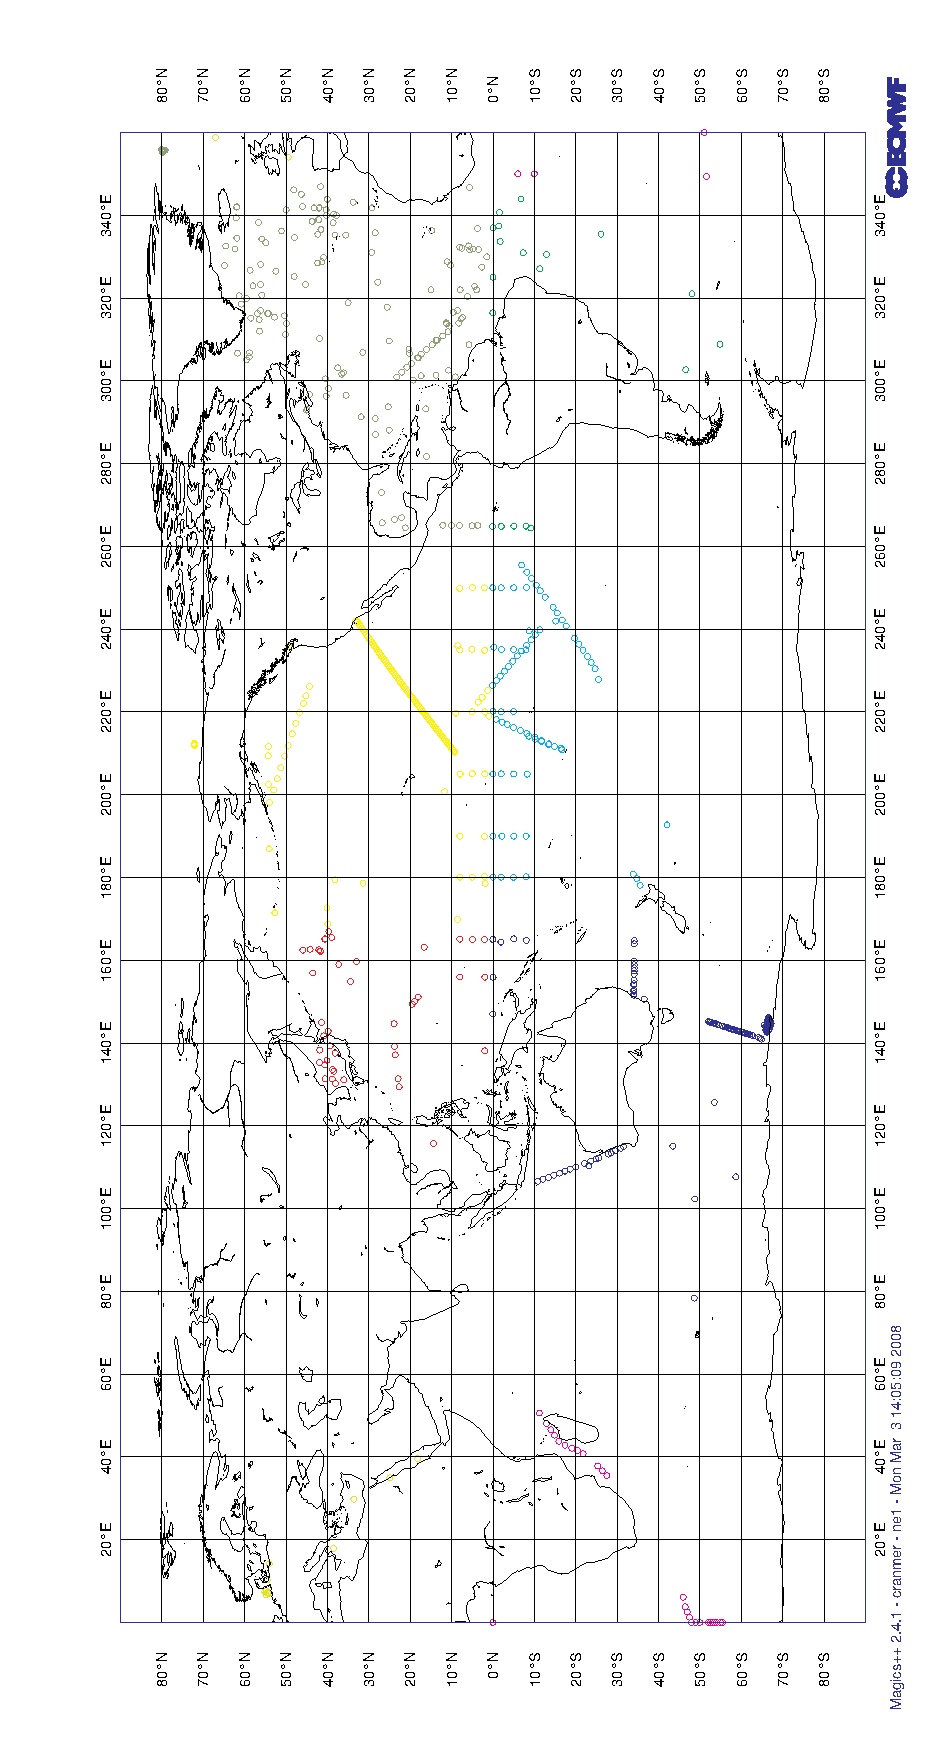
\includegraphics[width=10cm,height=12cm,angle=-90.]{./TexFiles/Figures/Fig_ASM_obsdist_local}
\caption{      \label{fig:obslocal}
Example of the distribution of observations with the geographical distribution of observational data.} 
\end{center}      \end{figure}
%>>>>>>>>>>>>>>>>>>>>>>>>>>>>

This is the simplest option in which the observations are distributed according 
to the domain of the grid-point parallelization. Figure~\ref{fig:obslocal}
shows an example of the distribution of the {\em in situ} data on processors 
with a different colour for each observation
on a given processor for a 4 $\times$ 2 decomposition with ORCA2. 
The grid-point domain decomposition is clearly visible on the plot.

The advantage of this approach is that all
information needed for horizontal interpolation is available without
any MPP communication. Of course, this is under the assumption that 
we are only using a $2 \times 2$ grid-point stencil for the interpolation 
(e.g., bilinear interpolation). For higher order interpolation schemes this
is no longer valid. A disadvantage with the above scheme is that the number of
observations on each processor can be very different. If the cost of
the actual interpolation is expensive relative to the communication of
data needed for interpolation, this could lead to load imbalance.

\subsubsection{Round-robin distribution of observations among processors}

%>>>>>>>>>>>>>>>>>>>>>>>>>>>>
\begin{figure}     \begin{center}
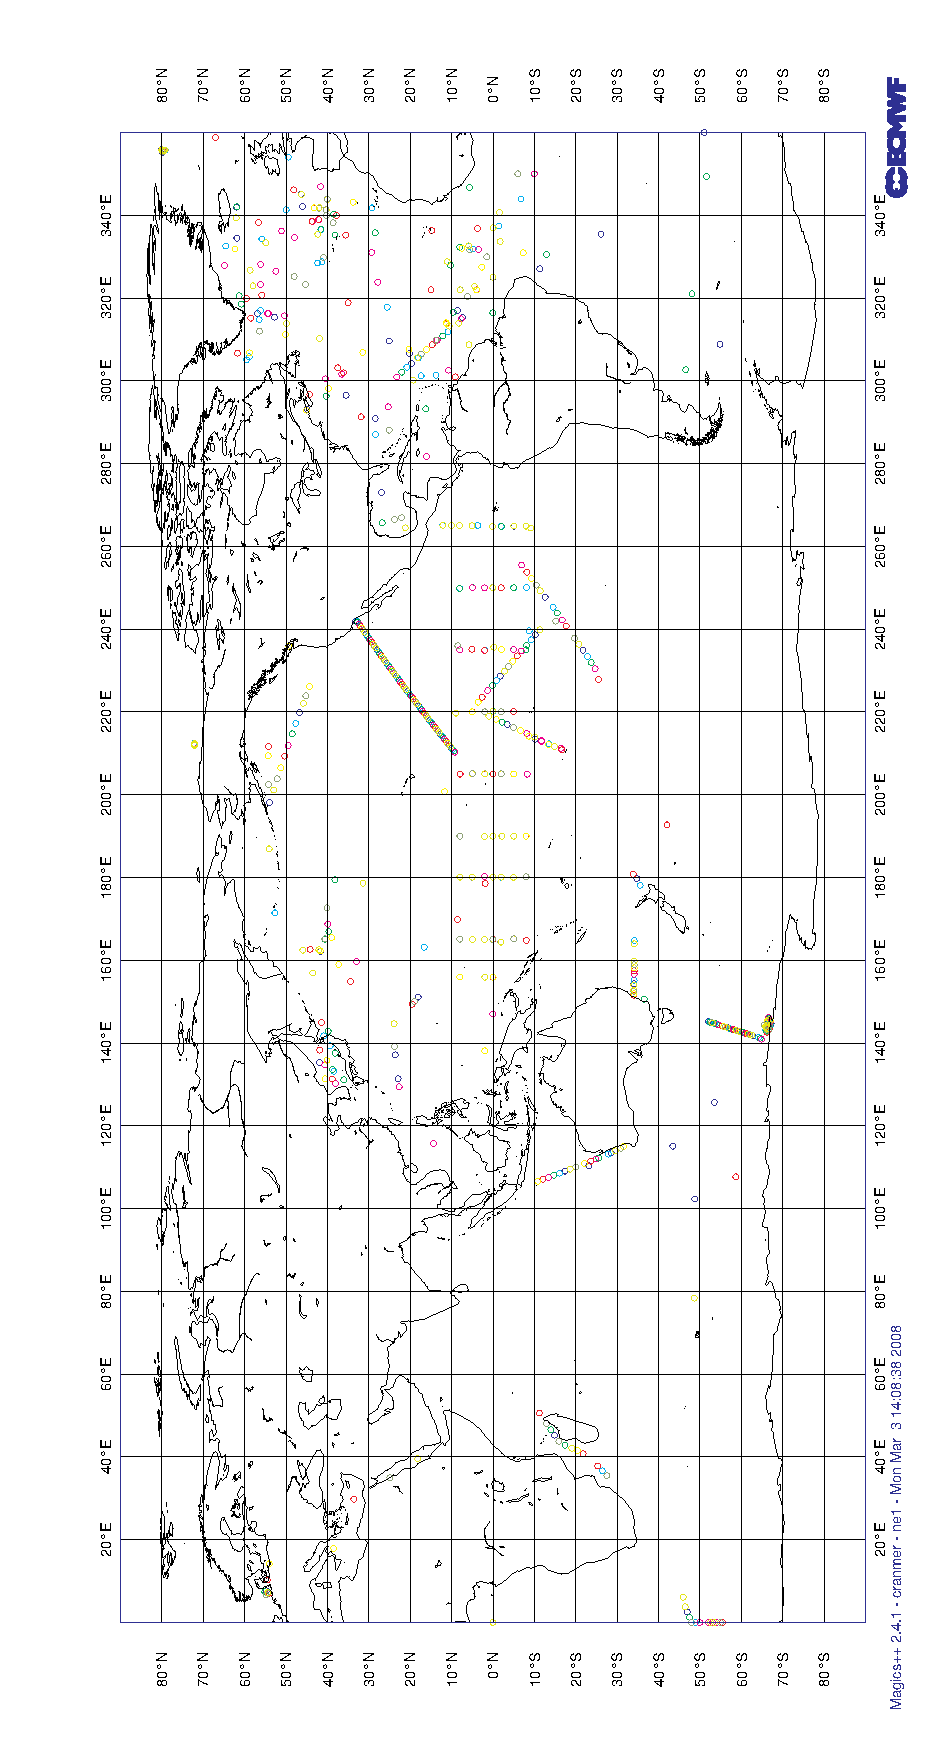
\includegraphics[width=10cm,height=12cm,angle=-90.]{./TexFiles/Figures/Fig_ASM_obsdist_global}
\caption{      \label{fig:obsglobal}
Example of the distribution of observations with the round-robin distribution of observational data.}
\end{center}     \end{figure}
%>>>>>>>>>>>>>>>>>>>>>>>>>>>>

An alternative approach is to distribute the observations equally
among processors and use message passing in order to retrieve 
the stencil for interpolation. The simplest distribution of the observations 
is to distribute them using a round-robin scheme. Figure~\ref{fig:obsglobal}
shows the distribution of the {\em in situ} data on processors for the
round-robin distribution of observations with a different colour for
each observation on a given processor for a 4 $\times$ 2 decomposition 
with ORCA2 for the same input data as in Fig.~\ref{fig:obslocal}.
The observations are now clearly randomly distributed on the globe.
In order to be able to perform horizontal interpolation in this case, 
a subroutine has been developed that retrieves any grid points in the 
global space.

\subsection{Vertical interpolation operator}

Vertical interpolation is achieved using either a cubic spline or
linear interpolation. For the cubic spline, the top and
bottom boundary conditions for the second derivative of the 
interpolating polynomial in the spline are set to zero.
At the bottom boundary, this is done using the land-ocean mask.

\newpage

% ================================================================
% Offline observation operator documentation
% ================================================================

%\usepackage{framed}

\section{Offline observation operator}
\label{OBS_ooo}

\subsection{Concept}

The obs oper maps model variables to observation space. It is possible to apply this mapping
without running the model. The software which performs this functionality is known as the
\textbf{offline obs oper}. The obs oper is divided into three stages. An initialisation phase,
an interpolation phase and an output phase. The implementation of which is outlined in the
previous sections. During the interpolation phase the offline obs oper populates the model
arrays by reading saved model fields from disk.

There are two ways of exploiting this offline capacity. The first is to mimic the behaviour of
the online system by supplying model fields at regular intervals between the start and the end
of the run. This approach results in a single model counterpart per observation. This kind of
usage produces feedback files the same file format as the online obs oper. 
The second is to take advantage of the offline setting in which multiple model counterparts can
be calculated per observation. In this case it is possible to consider all forecasts verifying
at the same time. By forecast, I mean any method which produces an estimate of physical reality
which is not an observed value. In the case of class 4 files this means forecasts, analyses, persisted
analyses and climatological values verifying at the same time. Although the class 4 file format
doesn't account for multiple ensemble members or multiple experiments per observation, it is possible
to include these components in the same or multiple files.

%--------------------------------------------------------------------------------------------------------
% offline_oper.exe 
%--------------------------------------------------------------------------------------------------------

\subsection{Using the offline observation operator}

\subsubsection{Building}

In addition to \emph{OPA\_SRC} the offline obs oper requires the inclusion
of the \emph{OOO\_SRC} directory. \emph{OOO\_SRC} contains a replacement \textbf{nemo.f90} and
\textbf{nemogcm.F90} which overwrites the resultant \textbf{nemo.exe}. This is the approach taken
by \emph{SAS\_SRC} and \emph{OFF\_SRC}.

%--------------------------------------------------------------------------------------------------------
% Running 
%--------------------------------------------------------------------------------------------------------
\subsubsection{Running}

The simplest way to use the executable is to edit and append the \textbf{ooo.nml} namelist to
a full NEMO namelist and then to run the executable as if it were nemo.exe. 

\subsubsection{Quick script}

A useful Python utility to control the namelist options can be found in \textbf{OBSTOOLS/OOO}. The
functions which locate model fields and observation files can be manually specified. The package
can be installed by appropriate use of the included setup.py script.

Documentation can be auto-generated by Sphinx by running \emph{make html} in the \textbf{doc} directory.

%--------------------------------------------------------------------------------------------------------
% Configuration section
%--------------------------------------------------------------------------------------------------------
\subsection{Configuring the offline observation operator}
The observation files and settings understood by \textbf{namobs} have been outlined in the online
obs oper section. In addition there are two further namelists wich control the operation of the offline
obs oper. \textbf{namooo} which controls the input model fields and \textbf{namcl4} which controls the
production of class 4 files. 

\subsubsection{Single field}

In offline mode model arrays are populated at appropriate time steps via input files.
At present, \textbf{tsn} and \textbf{sshn} are populated by the default read routines. 
These routines will be expanded upon in future versions to allow the specification of any
model variable. As such, input files must be global versions of the model domain with
\textbf{votemper}, \textbf{vosaline} and optionally \textbf{sshn} present.

For each field read there must be an entry in the \textbf{namooo} namelist specifying the
name of the file to read and the index along the \emph{time\_counter}. For example, to
read the second time counter from a single file the namelist would be.

\begin{alltt}
\tiny
\begin{verbatim} 
!----------------------------------------------------------------------
!       namooo Offline obs_oper namelist
!----------------------------------------------------------------------
!   ooo_files    specifies the files containing the model counterpart
!   nn_ooo_idx   specifies the time_counter index within the model file
&namooo
   ooo_files = "foo.nc"
   nn_ooo_idx = 2
/
\end{verbatim} 
\end{alltt}

\subsubsection{Multiple fields per run}

Model field iteration is controlled via \textbf{nn\_ooo\_freq} which specifies
the number of model steps at which the next field gets read. For example, if
12 hourly fields are to be interpolated in a setup where 288 steps equals 24 hours.

\begin{alltt}
\tiny
\begin{verbatim} 
!----------------------------------------------------------------------
!       namooo Offline obs_oper namelist
!----------------------------------------------------------------------
!   ooo_files    specifies the files containing the model counterpart
!   nn_ooo_idx   specifies the time_counter index within the model file
!   nn_ooo_freq  specifies number of time steps between read operations
&namooo
   ooo_files = "foo.nc" "foo.nc"
   nn_ooo_idx = 1 2
   nn_ooo_freq = 144
/
\end{verbatim} 
\end{alltt}

The above namelist will result in feedback files whose first 12 hours contain
the first field of foo.nc and the second 12 hours contain the second field.

%\begin{framed}
\textbf{Note} Missing files can be denoted as "nofile".
%\end{framed}

It is easy to see how a collection of fields taken fron a number of files 
at different indices can be combined at a particular frequency in time to 
generate a pseudo model evolution. As long as all that is needed is a single
model counterpart at a regular interval then namooo is all that needs to
be edited. However, a far more interesting approach can be taken in which
multiple forecasts, analyses, persisted analyses and climatologies are
considered against the same set of observations. For this a slightly more
complicated approach is needed. It is referred to as \emph{Class 4} since
it is the fourth metric defined by the GODAE intercomparison project.

%--------------------------------------------------------------------------------------------------------
% Class 4 file section
%--------------------------------------------------------------------------------------------------------
\subsubsection{Multiple model counterparts per observation a.k.a Class 4}

A generalisation of feedback files to allow multiple model components per observation. For a single
observation, as well as previous forecasts verifying at the same time there are also analyses, persisted
analyses and climatologies. 


The above namelist performs two basic functions. It organises the fields
given in \textbf{namooo} into groups so that observations can be matched
up multiple times. It also controls the metadata and the output variable
of the class 4 file when a write routine is called.

%\begin{framed}
\textbf{Note: ln\_cl4} must be set to \emph{.TRUE.} in \textbf{namobs} 
to use class 4 outputs.
%\end{framed}

\subsubsection{Class 4 naming convention}

The standard class 4 file naming convention is as follows.

\noindent
\linebreak
\textbf{\$\{prefix\}\_\$\{yyyymmdd\}\_\$\{sys\}\_\$\{cfg\}\_\$\{vn\}\_\$\{kind\}\_\$\{nproc\}.nc}

\noindent
\linebreak
Much of the namelist is devoted to specifying this convention. The
following namelist settings control the elements of the output
file names. Each should be specified as a single string of character data.

\begin{description}
\item[cl4\_prefix]
Prefix for class 4 files e.g. class4
\item[cl4\_date]
YYYYMMDD validity date
\item[cl4\_sys]
The name of the class 4 model system e.g. FOAM
\item[cl4\_cfg]
The name of the class 4 model configuration e.g. orca025
\item[cl4\_vn]
The name of the class 4 model version e.g. 12.0
\end{description}

\noindent
The kind is specified by the observation type internally to the obs oper. The processor
number is specified internally in NEMO. 

\subsubsection{Class 4 file global attributes}

Global attributes necessary to fulfill the class 4 file definition. These
are also useful pieces of information when collaborating with external
partners.

\begin{description}
\item[cl4\_contact]
Contact email for class 4 files.
\item[cl4\_inst]
The name of the producers institution.
\item[cl4\_cfg]
The name of the class 4 model configuration e.g. orca025
\item[cl4\_vn]
The name of the class 4 model version e.g. 12.0
\end{description}

\noindent
The obs\_type,
creation date and validity time are specified internally to the obs oper.

\subsubsection{Class 4 model counterpart configuration}

As seen previously it is possible to perform a single sweep of the
obs oper and specify a collection of model fields equally spaced 
along that sweep. In the class 4 case the single sweep is replaced
with multiple sweeps and a certain ammount of book keeping is
needed to ensure each model counterpart makes its way to the 
correct piece of memory in the output files.

\noindent
\linebreak
In terms of book keeping, the offline obs oper needs to know how many
full sweeps need to be performed. This is specified via the 
\textbf{cl4\_match\_len} variable and is the total number of model
counterparts per observation. For example, a 3 forecasts plus 3 persistence
fields plus an analysis field would be 7 counterparts per observation.

\begin{alltt}
\tiny
\begin{verbatim}
   cl4_match_len = 7
\end{verbatim}
\end{alltt}

Then to correctly allocate a class 4 file the forecast axis must be defined. This
is controlled via \textbf{cl4\_fcst\_len}, which in out above example would be 3.

\begin{alltt}
\tiny
\begin{verbatim}
   cl4_fcst_len = 3
\end{verbatim}
\end{alltt}

Then for each model field it is necessary to designate what class 4 variable and
index along the forecast dimension the model counterpart should be stored in the
output file. As well as a value for that lead time in hours, this will be useful
when interpreting the data afterwards. 

\begin{alltt}
\tiny
\begin{verbatim}
   cl4_vars = "forecast" "forecast" "forecast" "persistence" "persistence"
              "persistence" "best_estimate"
   cl4_fcst_idx = 1 2 3 1 2 3 1
   cl4_leadtime = 12 36 60 
\end{verbatim}
\end{alltt}

In terms of files and indices of fields inside each file the class 4 approach
makes use of the \textbf{namooo} namelist. If our fields are in separate files
with a single field per file our example inputs will be specified.

\begin{alltt}
\tiny
\begin{verbatim}
   ooo_files = "F.1.nc" "F.2.nc" "F.3.nc" "P.1.nc" "P.2.nc" "P.3.nc" "A.1.nc"
   nn_ooo_idx = 1 1 1 1 1 1 1
\end{verbatim}
\end{alltt}

When we combine all of the naming conventions, global attributes and i/o instructions
the class 4 namelist becomes.

\begin{alltt}
\tiny
\begin{verbatim}
!----------------------------------------------------------------------
!       namooo Offline obs_oper namelist
!----------------------------------------------------------------------
!   ooo_files    specifies the files containing the model counterpart
!   nn_ooo_idx   specifies the time_counter index within the model file
!   nn_ooo_freq  specifies number of time steps between read operations
&namooo
   ooo_files = "F.1.nc" "F.2.nc" "F.3.nc" "P.1.nc" "P.2.nc" "P.3.nc" "A.1.nc"
   nn_ooo_idx = 1 1 1 1 1 1 1
/
!----------------------------------------------------------------------
!       namcl4 Offline obs_oper class 4 namelist
!----------------------------------------------------------------------
!
!  Naming convention
!  -----------------
!  cl4_prefix    specifies the output file prefix
!  cl4_date      specifies the output file validity date
!  cl4_sys       specifies the model counterpart system
!  cl4_cfg       specifies the model counterpart configuration
!  cl4_vn        specifies the model counterpart version
!  cl4_inst      specifies the model counterpart institute
!  cl4_contact   specifies the file producers contact details
!
!  I/O specification
!  -----------------
!  cl4_vars      specifies the names of the output file netcdf variable
!  cl4_fcst_idx  specifies output file forecast index
!  cl4_fcst_len  specifies forecast axis length
!  cl4_match_len specifies number of unique matches per observation
!  cl4_leadtime  specifies the forecast axis lead time 
!
&namcl4
   cl4_match_len = 7
   cl4_fcst_len = 3
   cl4_fcst_idx = 1 2 3 1 2 3 1
   cl4_vars = "forecast" "forecast" "forecast" "persistence" "persistence"
              "persistence" "best_estimate"
   cl4_leadtime = 12 36 60
   cl4_prefix = "class4"
   cl4_date = "20130101"
   cl4_vn = "12.0"
   cl4_sys = "FOAM"
   cl4_cfg = "AMM7"
   cl4_contact = "example@example.com"
   cl4_inst = "UK Met Office"
/
\end{verbatim}
\end{alltt}

\subsubsection{Climatology interpolation}

The climatological counterpart is generated at the start of the run by restarting 
the model from climatology through appropriate use of \textbf{namtsd}. To override
the offline observation operator read routine and to take advantage of the restart
settings, specify the first entry in \textbf{cl4\_vars} as "climatology". This will then
pipe the restart from climatology into the output class 4 file. As in every other
class 4 matchup the input file, input index and output index must be specified.
These can be replaced with dummy data since they are not used but they must be
present to cycle through the matchups correctly. 

\subsection{Advanced usage}

In certain cases it may be desirable to include both multiple model fields per
observation window with multiple match ups per observation. This can be achieved
by specifying \textbf{nn\_ooo\_freq} as well as the class 4 settings. Care must
be taken in generating the ooo\_files list such that the files are arranged into
consecutive blocks of single match ups. For example, 2 forecast fields 
of 12 hourly data would result in 4 separate read operations but only 2 write
operations, 1 per forecast.

\begin{alltt}
\tiny
\begin{verbatim}
   ooo_files = "F1.nc" "F1.nc" "F2.nc" "F2.nc"
...
   cl4_fcst_idx = 1 2
\end{verbatim}
\end{alltt}

The above notation reveals the internal split between match up iterators and file
iterators. This technique has not been used before so experimentation is needed
before results can be trusted.




\newpage

\section{Observation Utilities}
\label{OBS_obsutils}

Some tools for viewing and processing of observation and feedback files are provided in the
NEMO repository for convenience. These include OBSTOOLS which are a collection of Fortran
programs which are helpful to deal with feedback files. They do such tasks as observation file
conversion, printing of file contents, some basic statistical analysis of feedback files. The
other tool is an IDL program called dataplot which uses a graphical interface to visualise
observations and feedback files. OBSTOOLS and dataplot are described in more detail below.  

\subsection{Obstools}

A series of Fortran utilities is provided with NEMO called OBSTOOLS. This are helpful in
handling observation files and the feedback file output from the NEMO observation operator.
The utilities are as follows

\subsubsection{c4comb}

The program c4comb combines multiple class 4 files produced by individual processors in an
MPI run of NEMO offline obs\_oper into a single class 4 file. The program is called in the following way:

\begin{alltt}
\footnotesize
\begin{verbatim}
c4comb.exe outputfile inputfile1 inputfile2 ...
\end{verbatim}
\end{alltt}

\subsubsection{corio2fb}

The program corio2fb converts profile observation files from the Coriolis format to the
standard feedback format. The program is called in the following way:

\begin{alltt}
\footnotesize
\begin{verbatim}
corio2fb.exe outputfile inputfile1 inputfile2 ...
\end{verbatim}
\end{alltt}

\subsubsection{enact2fb}

The program enact2fb converts profile observation files from the ENACT format to the standard
feedback format. The program is called in the following way:

\begin{alltt}
\footnotesize
\begin{verbatim}
enact2fb.exe outputfile inputfile1 inputfile2 ...
\end{verbatim}
\end{alltt}

\subsubsection{fbcomb}

The program fbcomb combines multiple feedback files produced by individual processors in an
MPI run of NEMO into a single feedback file. The program is called in the following way:

\begin{alltt}
\footnotesize
\begin{verbatim}
fbcomb.exe outputfile inputfile1 inputfile2 ...
\end{verbatim}
\end{alltt}

\subsubsection{fbmatchup}

The program fbmatchup will match observations from two feedback files. The program is called
in the following way:

\begin{alltt}
\footnotesize
\begin{verbatim}
fbmatchup.exe outputfile inputfile1 varname1 inputfile2 varname2 ...
\end{verbatim}
\end{alltt}


\subsubsection{fbprint}

The program fbprint will print the contents of a feedback file or files to standard output.
Selected information can be output using optional arguments. The program is called in the
following way:

\begin{alltt}
\footnotesize
\begin{verbatim}
fbprint.exe [options] inputfile

options:
     -b            shorter output
     -q            Select observations based on QC flags
     -Q            Select observations based on QC flags
     -B            Select observations based on QC flags
     -u            unsorted
     -s ID         select station ID  
     -t TYPE       select observation type
     -v NUM1-NUM2  select variable range to print by number 
                      (default all)
     -a NUM1-NUM2  select additional variable range to print by number 
                      (default all)
     -e NUM1-NUM2  select extra variable range to print by number 
                      (default all)
     -d            output date range
     -D            print depths
     -z            use zipped files
\end{verbatim}
\end{alltt}

\subsubsection{fbsel}

The program fbsel will select or subsample observations. The program is called in the
following way:

\begin{alltt}
\footnotesize
\begin{verbatim}
fbsel.exe <input filename> <output filename>
\end{verbatim}
\end{alltt}

\subsubsection{fbstat}

The program fbstat will output summary statistics in different global areas into a number of
files. The program is called in the following way:

\begin{alltt}
\footnotesize
\begin{verbatim}
fbstat.exe [-nmlev] <filenames>
\end{verbatim}
\end{alltt}

\subsubsection{fbthin}

The program fbthin will thin the data to 1 degree resolution. The code could easily be
modified to thin to a different resolution. The program is called in the following way:

\begin{alltt}
\footnotesize
\begin{verbatim}
fbthin.exe inputfile outputfile
\end{verbatim}
\end{alltt}

\subsubsection{sla2fb}

The program sla2fb will convert an AVISO SLA format file to feedback format. The program is
called in the following way:

\begin{alltt}
\footnotesize
\begin{verbatim}
sla2fb.exe [-s type] outputfile inputfile1 inputfile2 ...

Option:
     -s            Select altimeter data_source
\end{verbatim}
\end{alltt}

\subsubsection{vel2fb}

The program vel2fb will convert TAO/PIRATA/RAMA currents files to feedback format. The program
is called in the following way:

\begin{alltt}
\footnotesize
\begin{verbatim}
vel2fb.exe outputfile inputfile1 inputfile2 ...
\end{verbatim}
\end{alltt}

\subsection{building the obstools}

To build the obstools use in the tools directory use ./maketools -n OBSTOOLS -m [ARCH].

\subsection{Dataplot}

An IDL program called dataplot is included which uses a graphical interface to visualise
observations and feedback files. It is possible to zoom in, plot individual profiles and
calculate some basic statistics. To plot some data run IDL and then:
\begin{alltt}
\footnotesize
\begin{verbatim}
IDL> dataplot, "filename"
\end{verbatim}
\end{alltt}

To read multiple files into dataplot, for example multiple feedback files from different
processors or from different days, the easiest method is to use the spawn command to generate
a list of files which can then be passed to dataplot.
\begin{alltt}
\footnotesize
\begin{verbatim}
IDL> spawn, 'ls profb*.nc', files
IDL> dataplot, files
\end{verbatim}
\end{alltt}

Fig~\ref{fig:obsdataplotmain} shows the main window which is launched when dataplot starts.
This is split into three parts. At the top there is a menu bar which contains a variety of
drop down menus. Areas - zooms into prespecified regions; plot - plots the data as a
timeseries or a T-S diagram if appropriate; Find - allows data to be searched; Config - sets
various configuration options.

The middle part is a plot of the geographical location of the observations. This will plot the
observation value, the model background value or observation minus background value depending
on the option selected in the radio button at the bottom of the window. The plotting colour
range can be changed by clicking on the colour bar. The title of the plot gives some basic
information about the date range and depth range shown, the extreme values, and the mean and
rms values. It is possible to zoom in using a drag-box. You may also zoom in or out using the
mouse wheel.

The bottom part of the window controls what is visible in the plot above. There are two bars
which select the level range plotted (for profile data). The other bars below select the date
range shown. The bottom of the figure allows the option to plot the mean, root mean square,
standard deviation or mean square values. As mentioned above you can choose to plot the
observation value, the model background value or observation minus background value. The next
group of radio buttons selects the map projection. This can either be regular latitude
longitude grid, or north or south polar stereographic. The next group of radio buttons will
plot bad observations, switch to salinity and plot density for profile observations. The
rightmost group of buttons will print the plot window as a postscript, save it as png, or exit
from dataplot.

%>>>>>>>>>>>>>>>>>>>>>>>>>>>>
\begin{figure}     \begin{center}
%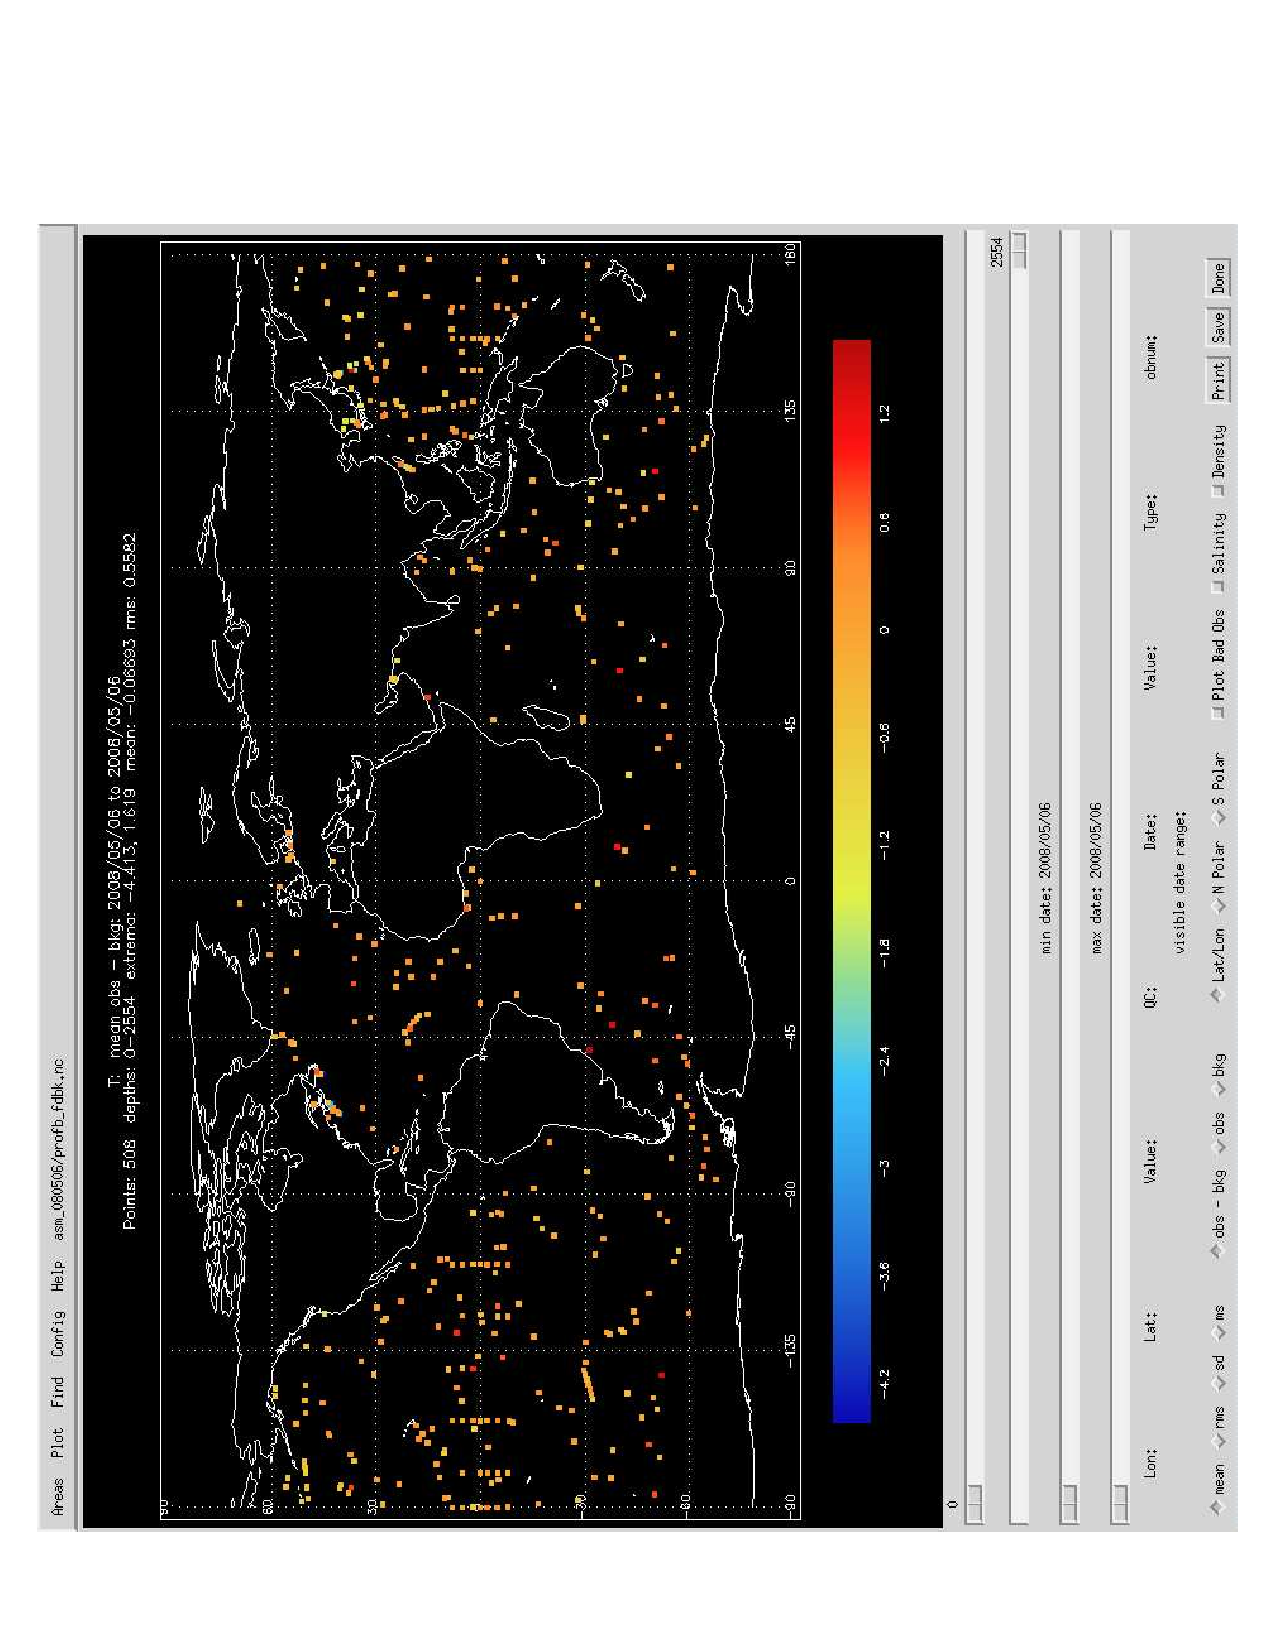
\includegraphics[width=10cm,height=12cm,angle=-90.]{./TexFiles/Figures/Fig_OBS_dataplot_main}
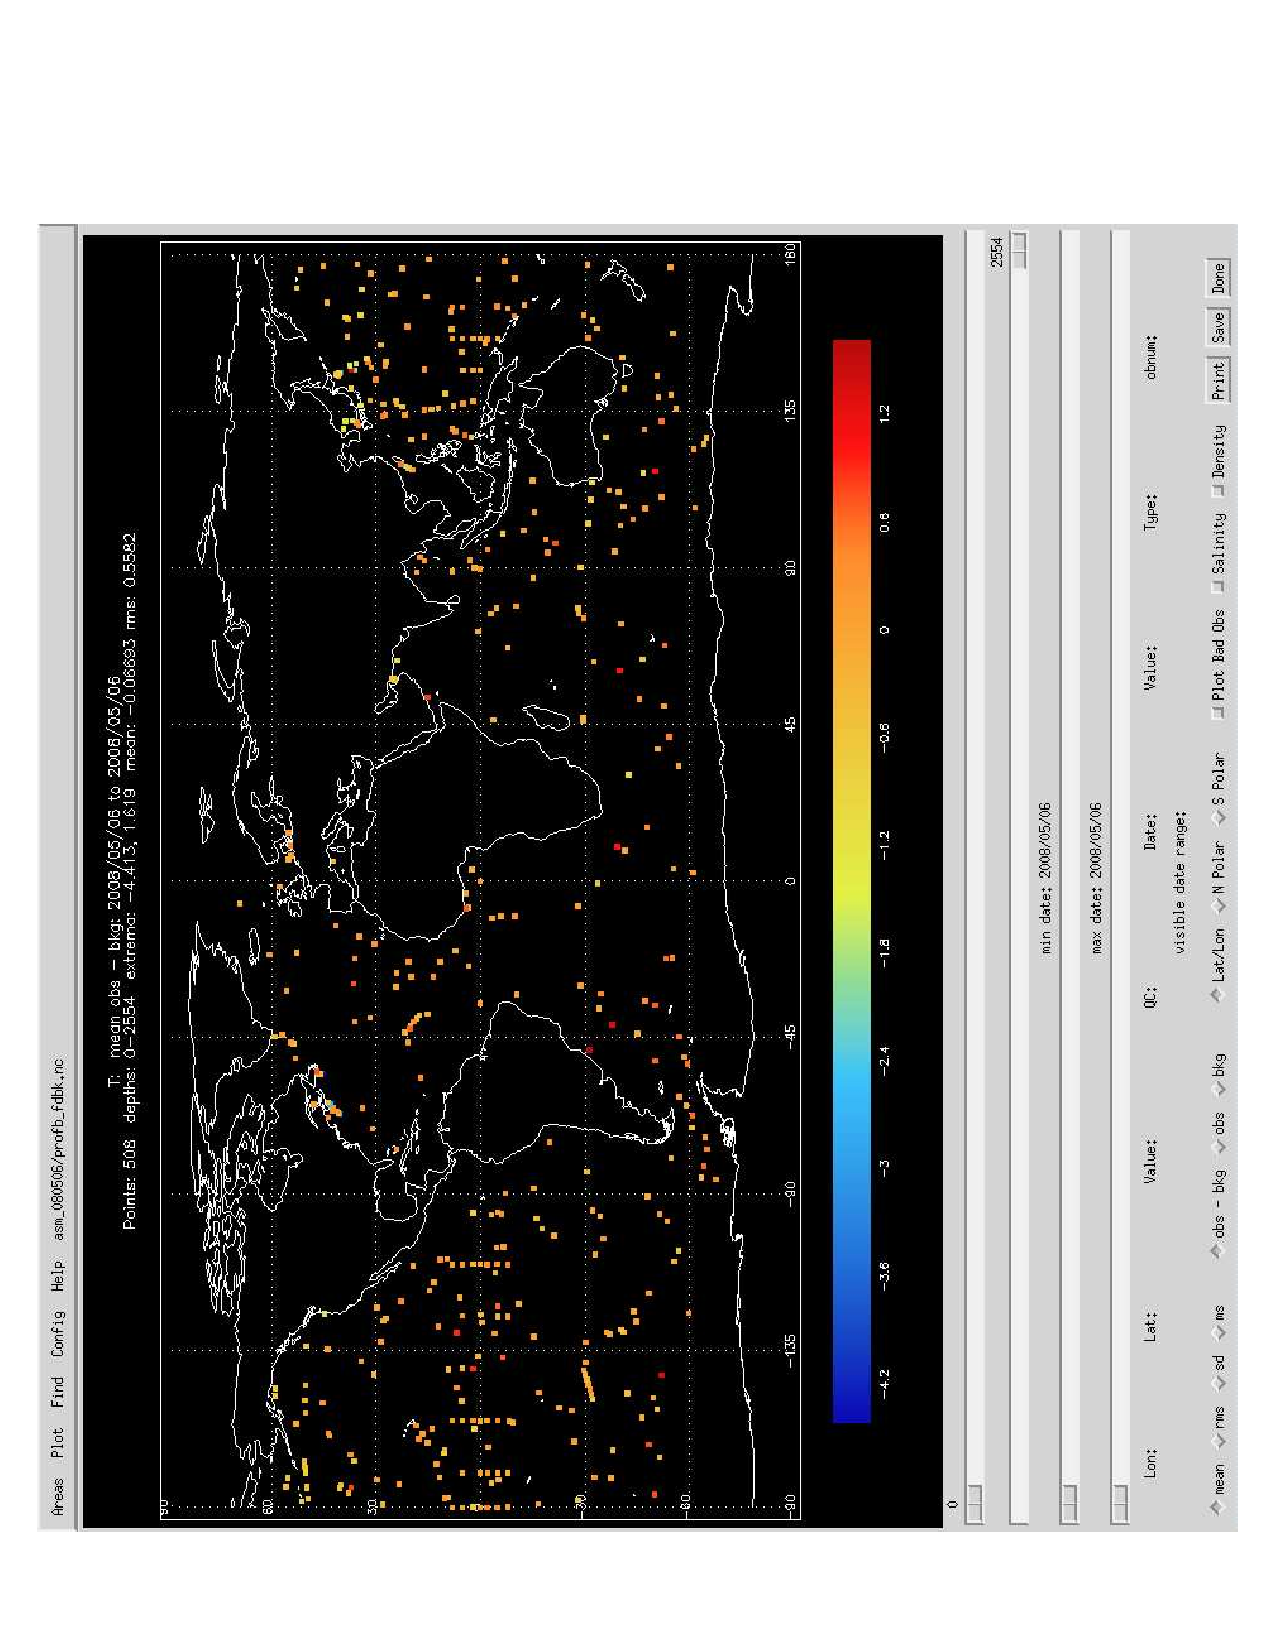
\includegraphics[width=9cm,angle=-90.]{./TexFiles/Figures/Fig_OBS_dataplot_main}
\caption{      \label{fig:obsdataplotmain}
Main window of dataplot.}
\end{center}     \end{figure}
%>>>>>>>>>>>>>>>>>>>>>>>>>>>>

If a profile point is clicked with the mouse button a plot of the observation and background
values as a function of depth (Fig~\ref{fig:obsdataplotprofile}).

%>>>>>>>>>>>>>>>>>>>>>>>>>>>>
\begin{figure}     \begin{center}
%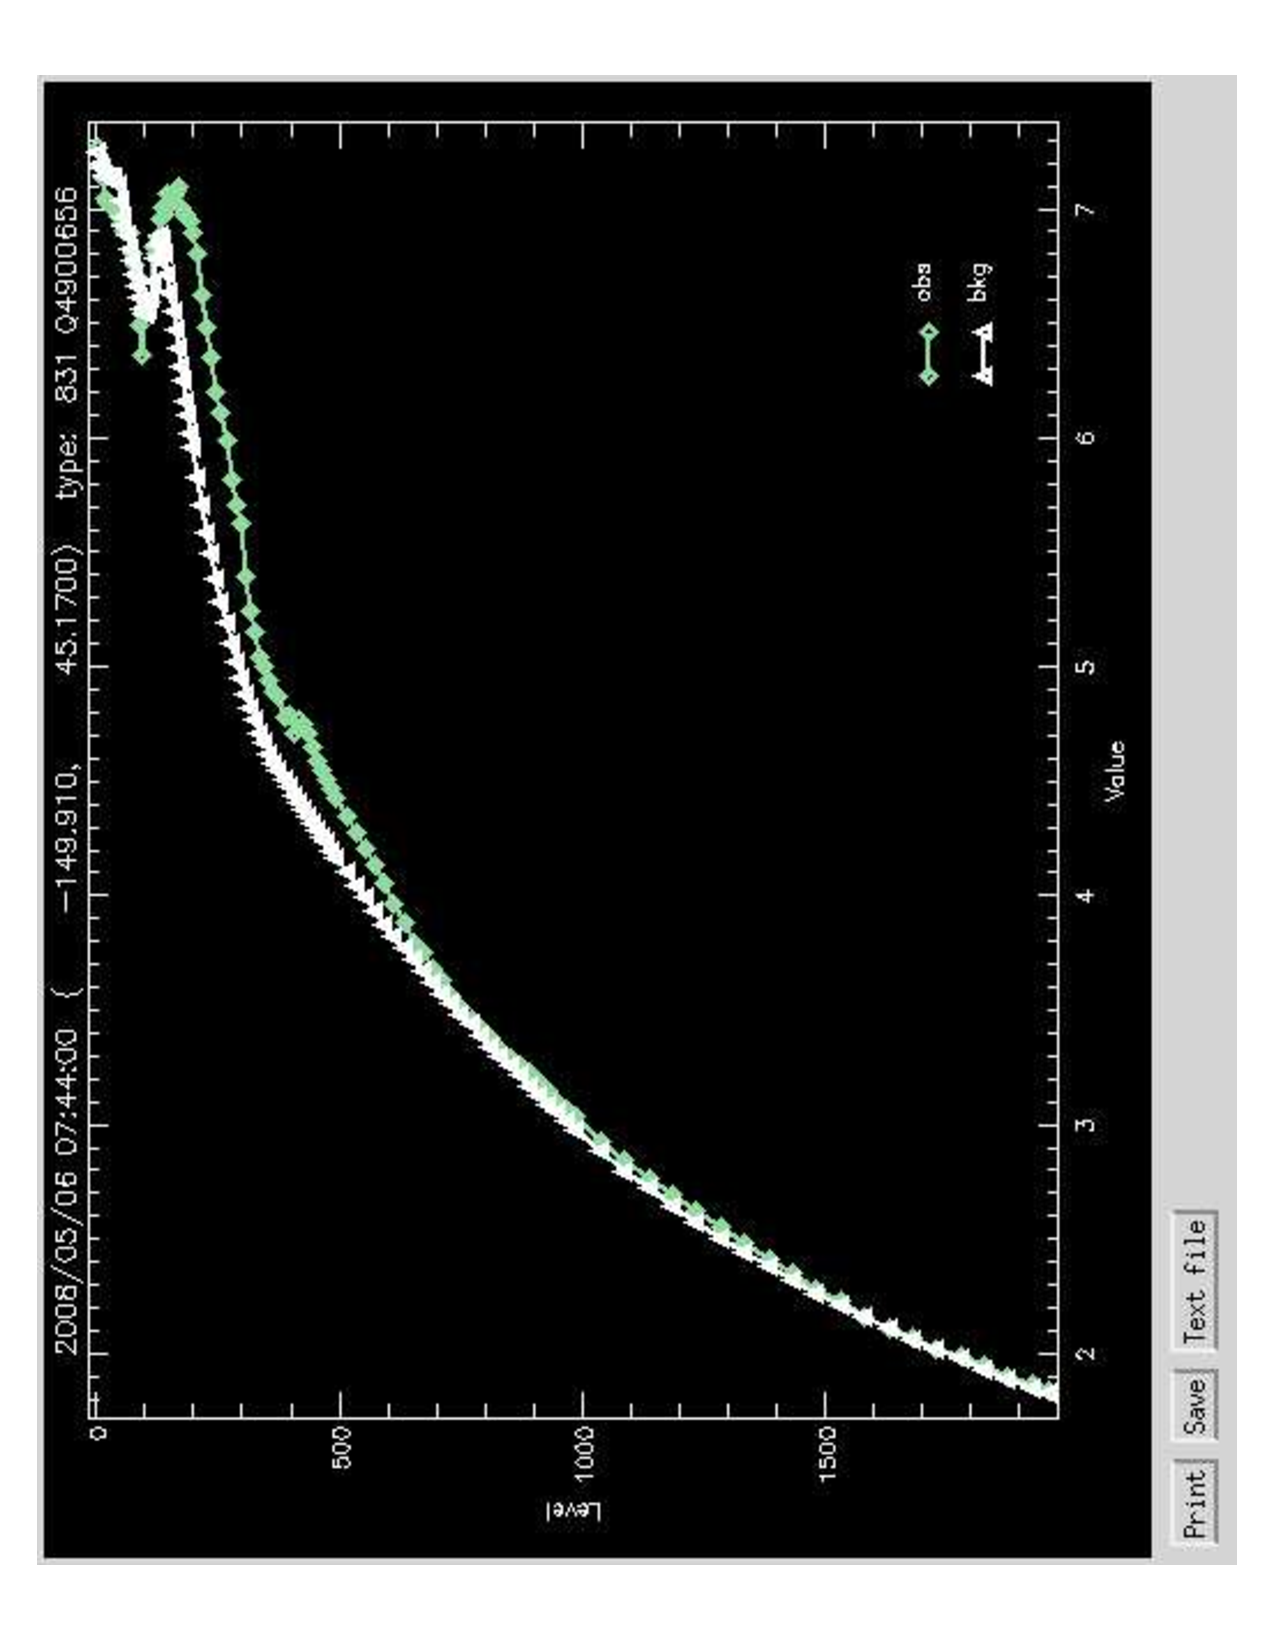
\includegraphics[width=10cm,height=12cm,angle=-90.]{./TexFiles/Figures/Fig_OBS_dataplot_prof}
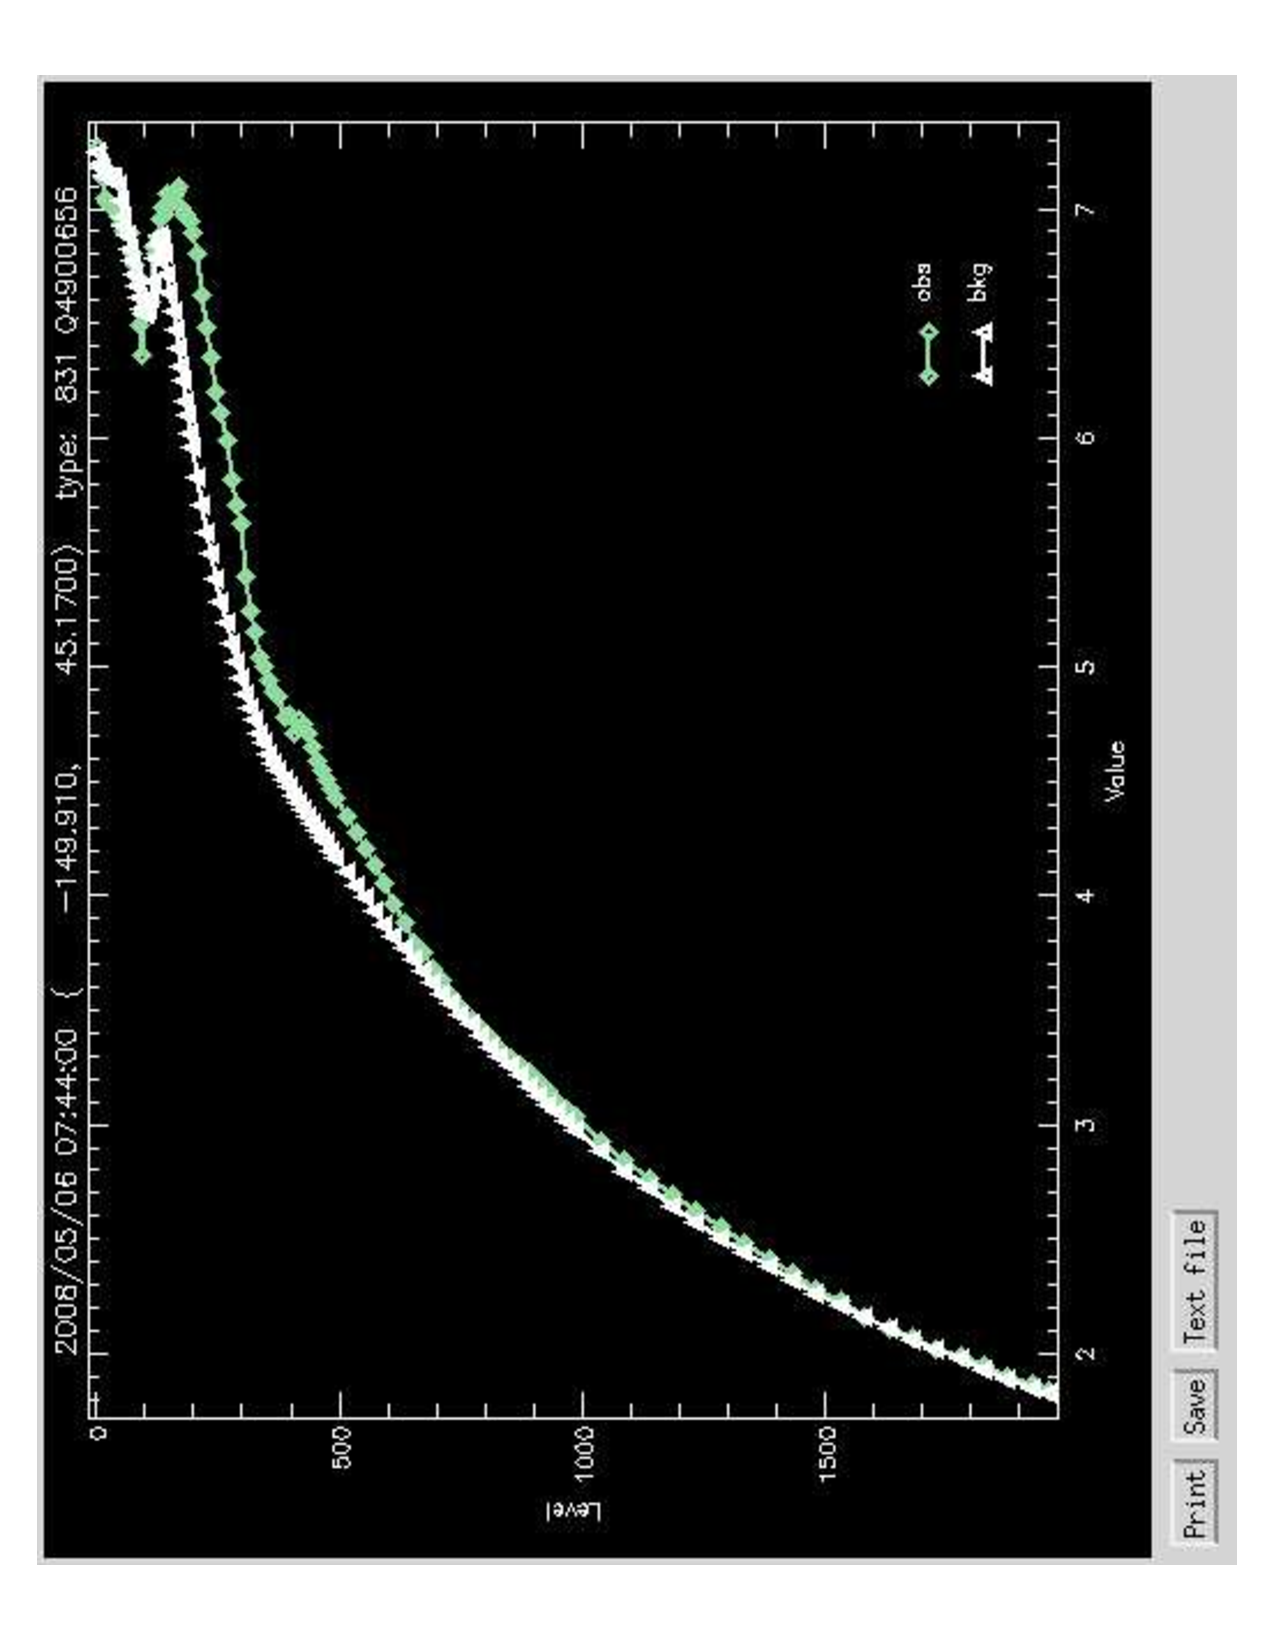
\includegraphics[width=7cm,angle=-90.]{./TexFiles/Figures/Fig_OBS_dataplot_prof}
\caption{      \label{fig:obsdataplotprofile}
Profile plot from dataplot produced by right clicking on a point in the main window.}
\end{center}     \end{figure}
%>>>>>>>>>>>>>>>>>>>>>>>>>>>>




